\chapter{程式講解}
\section{程式講解}
\begin{figure}[hbt!]
\begin{center}
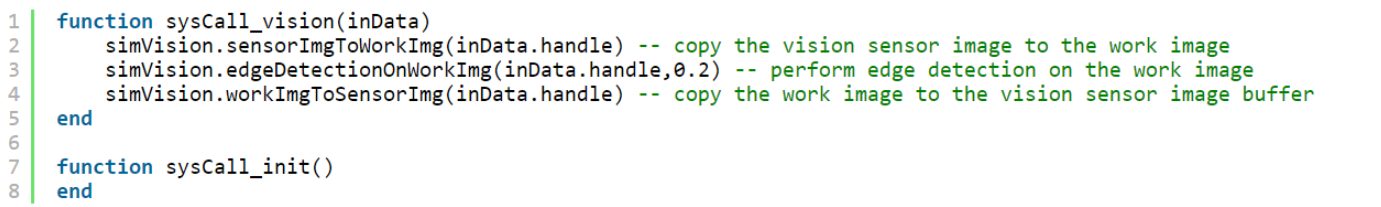
\includegraphics[width=16cm]{程式講解1}
\caption{\Large 程式講解}\label{程式講解}
\end{center}
\end{figure} 
首先這是一個Lua語言,在CoppeliaSim仿真環境中運行。該腳本定義了兩個函數:sysCallinit和sysCallvision。
\\
sysCallinit函數是仿真環境初始化時自動調用的函數,該函數目前是空的,即不執行任何操作。
\\
sysCallvision函數是CoppeliaSim的視覺模組塊(VisionModule)在每次運行時會調用的函數,該函數的作用是對視覺傳感器的圖像進行邊緣檢測(edge detection)。\\具體來說,函數中的三個函數調用分別為:
\begin{itemize}
%=----------simVision.sensorImgToWorkImg----------=%
\item simVision.sensorImgToWorkImg (圖.\ref{程式講解}):\\
將視覺傳感器的圖像複製到工作圖像中。\\
%=----------simVision.edgeDetectionOnWorkImg----------=%
\item simVision.edgeDetectionOnWorkImg (圖.\ref{程式講解}):\\
對工作圖像進行邊緣檢測,檢測閾值為0.2。\\
%=----------simVision.workImgToSensorImg----------=%
\item simVision.edgeDetectionOnWorkImg (圖.\ref{程式講解}):\\
將處理後的工作圖像複製回視覺傳感器的圖像緩衝區中。\\
其中,inData是一個包含了視覺模組塊的一些信息的table對象,例如handle(視覺傳感器的句柄)等。simVision是CoppeliaSim中提供的用於處理視覺相關任務的庫。\\
\end{itemize}
